\documentclass[10pt]{scrartcl}

\usepackage[utf8]{inputenc}
\usepackage{tabularx}
\usepackage[ngerman]{babel}
\usepackage[automark]{scrpage2}
\usepackage{amsmath,amssymb,amstext}
%\usepackage{mathtools}

\usepackage[]{enumerate}
\usepackage{graphicx}
\usepackage{lastpage}
\usepackage[perpage,para,symbol*]{footmisc}
\usepackage{listings}
\usepackage{color}
\usepackage{textcomp}
\definecolor{listinggray}{gray}{0.9}
\definecolor{lbcolor}{rgb}{0.9,0.9,0.9}
\lstset{
	backgroundcolor=\color{lbcolor},
	tabsize=4,
	rulecolor=,
	language=matlab,
        basicstyle=\scriptsize,
        upquote=true,
        aboveskip={1.5\baselineskip},
        columns=fixed,
        showstringspaces=false,
        extendedchars=true,
        breaklines=true,
        prebreak = \raisebox{0ex}[0ex][0ex]{\ensuremath{\hookleftarrow}},
        frame=single,
        showtabs=false,
        showspaces=false,
        showstringspaces=false,
        identifierstyle=\ttfamily,
        keywordstyle=\color[rgb]{0,0,1},
        commentstyle=\color[rgb]{0.133,0.545,0.133},
        stringstyle=\color[rgb]{0.627,0.126,0.941},
}
\usepackage[pdfborder={0 0 0},colorlinks=false]{hyperref}
\usepackage[numbers,square]{natbib}
\usepackage{float}

\lstset{numbers=left, numberstyle=\tiny, numbersep=5pt, breaklines=true, showstringspaces=false} 

%changehere
\def\titletext{Praktikum 3}
\def\titletextshort{Praktikum 3}
\author{Oliver Steenbuck, Karolina Bernat}

\title{\titletext}

%changehere Datum der Übung
\date{12.12.2012}

\pagestyle{scrheadings}
%changehere
\ihead{MT, Pareigis}
\ifoot{Generiert am:\\ \today}

\cfoot{Karolina Bernat, Oliver Steenbuck}


\ohead[]{\titletextshort}
\ofoot[]{{\thepage} / \pageref{LastPage}}

\setlength{\parindent}{0.0in}
\setlength{\parskip}{0.1in}

\begin{document}
\maketitle
\setcounter{tocdepth}{3}
\tableofcontents
\listoffigures
\lstlistoflistings


\section{Rakete}
	Der zu simulierende Raketenflug besteht aus 3 Teilen. Die zu simulierende Rakete aus 2 Stufen, die nacheinander die Rakete antreiben und danach abgeworfen werden.
	Es soll die Geschwindigkeit sowie die Höhe jeweils von Stufe 1 und Stufe 2 simuliert werden.
	

	\subsection{StufenGemeinsam} \label{sec:stufenGemeinsam}
	In dieser Phase wird die gesamte Rakete durch Stufe 1 beschleunigt.
	
	Die Masse der Rakete ergibt sich also aus.
	\begin{align} 
	m_{\text{Rakete}} = m_1 + m_2
	\end{align}

	Die Schubkraft der Rakete ergibt sich hier durch
	\begin{align}
	F_s = \text{Durchsatz}_1 * \text{SchubProDurchsatz}
	\end{align}

	Die Erdanziehung, die auf die Rakete wirkt, kann durch die untenstehende Formel berechnet werden, wobei:\\ $r = \text{Erdradius} + \text{Entfernung der Rakete von der Erde}$
	\begin{align}
	F_e = \frac{G * m_{\text{erde}} * m_{\text{Rakete}}}{r^2}
	\end{align}
	
	Gegeben die oben berechneten Werten können wir nun die Beschleunigung der Rakete berechnen durch:
	\begin{align}
	a_{\text{Rakete}} = \frac{F_s - F_e}{m_{\text{Rakete}}}
	\end{align}
	
	\subsection{Stufe 2}
	In dieser Phase ist Stufe 1 ausgebrannt und beginnt zur Erde zurückzufallen. Während dessen besteht die Rakete nur noch aus Stufe 2 , die auch den Antrieb liefert. Beide Stufen sind hier also getrennt zu betrachten.
	
	\subsubsection{Stufe 2}
	Stufe 2 wird hier weiter als Rakete bezeichnet, somit ergeben sich unter Anpassung der Formeln aus \ref{sec:stufenGemeinsam} folgende neue Formeln zur Berechnung des Raketenfluges.
	
	Die Masse der Rakete besteht nur noch aus der Masse der zweiten Stufe.
	\begin{align} 
	m_{\text{Rakete}} = m_2
	\end{align}

	Die Schubkraft der Rakete ergibt sich jetzt durch die zweite Stufe.
	\begin{align}
	F_s = \text{Durchsatz}_2 * \text{SchubProDurchsatz}
	\end{align}

	Die Erdanziehung, die auf die Rakete wirkt, kann unverändert berechnet werden durch:
	\begin{align}
	F_e = \frac{G * m_{\text{erde}} * m_{\text{Rakete}}}{r_{\text{erde}}^2}
	\end{align}
	
	Für die Beschleunigung der Rakete gilt weiterhin:
	\begin{align}
	a_{\text{Rakete}} = \frac{F_s - F_e}{m_{\text{Rakete}}}
	\end{align}	
	
	\subsubsection{Stufe 1}
	Die abgetrennte Stufe 1 \textit{fliegt} jetzt antriebslos, also nur noch durch die Erdanziehung beeinflusst, weiter.
	Ihre Beschleunigung kann also wie oben modelliert werden: 
	
	\begin{align}
	a_{\text{Stufe 1}} = \frac{F_s - F_{e1}}{m_1}
	\end{align}		
	
	Wobei $F_s$ die Schubkraft vernachlässigt werden kann, wodurch sich die bereinigte Formel ergibt:
	\begin{align}
	a_{\text{Stufe 1}} = \frac{- F_{e1}}{m_1}
	\end{align}			
	
	
	
	\subsection{Antrieblos}
	Beide Stufen \textit{fliegen} jetzt antriebslos und damit nur noch unter Auswirkung der Erdanziehung.
	Es gelten also folgende Formeln für beide Stufen:
	\begin{align}
	a_{\text{Stufe 1}} = \frac{- F_{e1}}{m_1}
	\end{align}	
	
	Und:
	\begin{align}
	a_{\text{Stufe 2}} = \frac{- F_{e2}}{m_2}
	\end{align}	

	\subsection{Ergebnisse}
	Bei den folgenden Startwerten ergeben sich die unten (Abbildung \ref{pic:rakete}) dargestellten Verläufe von Geschwindigkeit und Höhe:
	\begin{description}
		\item[m1\_leer] 500
		\item[m2\_leer] 1000
		\item[St1\_Treibstoff] 4000
		\item[St2\_Treibstoff] 1500
		\item[Durchsatz\_1] 20
		\item[Durchsatz\_2] 15
		\item[SchubProDurchsatz] 4000
	\end{description}
	
	\subsubsection{Graphen}	
	\begin{figure}[htbp]
		\centering
		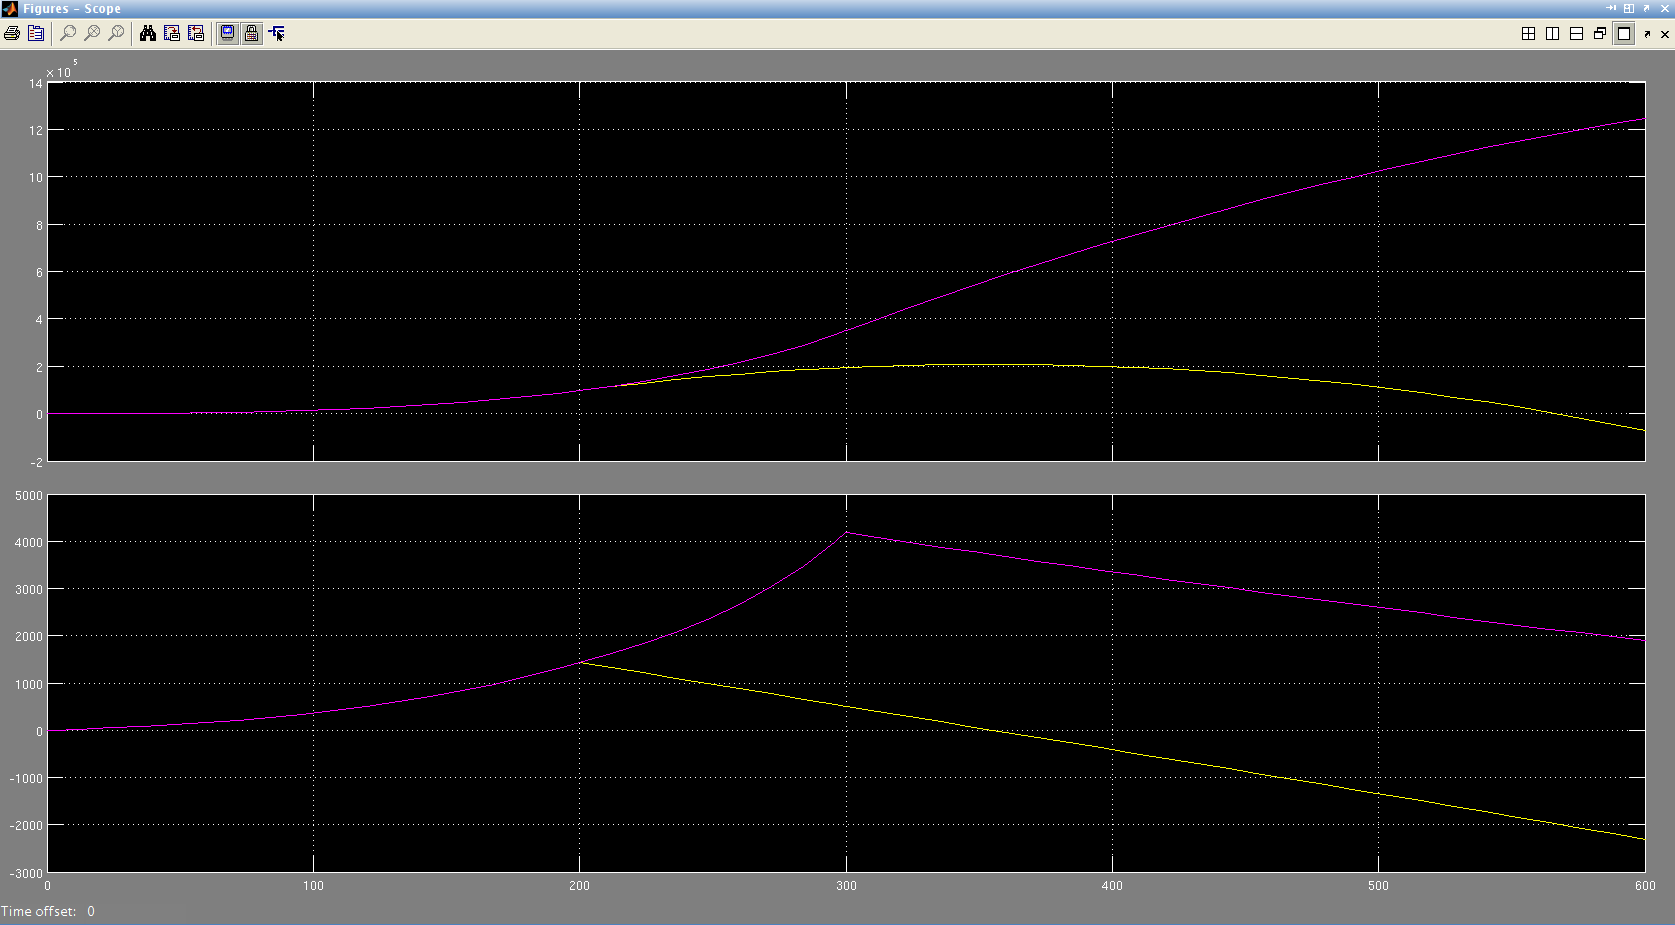
\includegraphics[scale=0.25]{ScreenshotRakete.png}
		\caption{Höhe und Geschwindigkeit der Rakete}
		\label{pic:rakete}
	\end{figure}

	\subsubsection{Auswertung}
	Wir können sehen, dass Stufe 1 nach der Trennung durch die Erdgravitation abgebremst wird und ca. 550 Sekunden nach dem Start wieder auf dem Boden aufschlägt. Stufe 2 steigt über die gesamte Simulationszeit weiter auf, ab Sekunde 300 sinkt nach dem Übergang in die antriebslose Phase auch die Geschwindigkeit von Stufe 2.
	
	Die maximale Höhe, die durch ein Raketenteil während der Simulation erreicht wird ist ca. 1250 km durch Stufe 2. Die maximale Geschwindigkeit, beim Übertritt in den antriebslosen Flug beträgt ca. $4100 \frac{m}{s}$
	Erhöht man die Simulationszeit auf 900 Sekunden erreicht Stufe 2 ihren maximalen Aufstieg (Punkt bei dme die Geschwindigkeit 0 wird) bei ca. 1510km.
	
	\subsection{Schaltung}
	\begin{figure}[htbp]
		\centering
		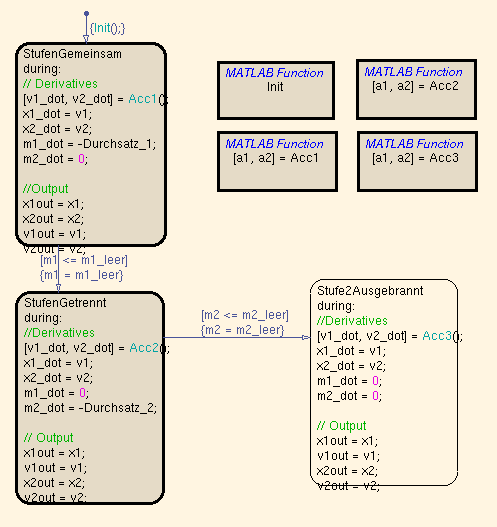
\includegraphics[scale=0.55]{ScreenshotRaketeAutomat.png}
		\caption{Stateflow Rakete}
		\label{pic:stateflowRakete}
	\end{figure}

	
\section{Tisch}	
Zu simulieren ist ein schiefer Flippertisch mit 3 Wänden und einem zylindrischem Hindernis. Gegeben sind die Eckpunkte der (verbundenen) Wände durch die Vektoren $P_{1..4}$ und die Position des Zylinderhindernises bei $P_{Zy}$. Auf die zu Beginn am Punkt $(4,5)$stillstehende Kugel wirkt eine konstante Beschleunigung von $g=1\frac{m}{s}$ nach unten. 
		
	\subsection{Automat}	
	\begin{figure}[htbp]
		\centering
		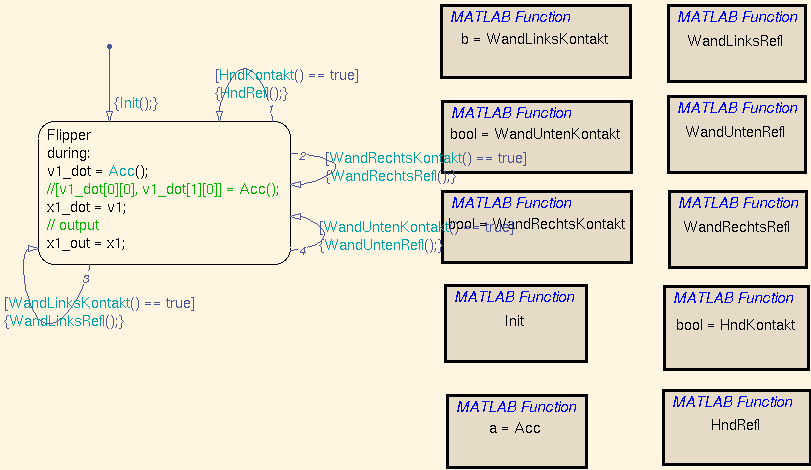
\includegraphics[scale=0.55]{ScreenshotFlipperAutomat.png}
		\caption{Stateflow Flipper}
		\label{pic:stateflowFlipper}
	\end{figure}
		
	\subsection{Modellierung}
	Im folgenden sind beispielhaft die Funktionen dargestellt, die den Kontakt und die Reflexion von der unteren Wand modellieren.
	
	Kontakt:
	\begin{lstlisting}[tabsize=2, frame=single, label=Stiff, caption={WandUntenKontakt}]
	function bool = WandUntenKontakt
    bool = false;
    
    abstand = (x1 - p2)' * n2;  % Abstand von der Achse (p2, p3) in Normalenrichtung
    richtung = v1' * n2;        % Bewegungsrichtung der Kugel relativ zu Normalenrichtung
    
    if ((abstand < R) && (richtung < 0))
        bool = true;
    end
end
	\end{lstlisting}		

Reflexion:
\begin{lstlisting}[tabsize=2, frame=single, label=Stiff, caption={WandUntenReflexion}]
	function WandUntenRefl
    vt = v1' * t2;
    vn = v1' * n2;
    
    v1 = (vt' * t2) - (vn' * n2);
end
	\end{lstlisting}


\end{document}

